\chapter{Methodology}

This chapter presents the methodology adopted for the development of this thesis.

\section{Material}

To develop the Cart-OnePiece a specific set of software and hardware tools was utilized. The environment was built using the CARLA simulator version 0.9.16 \cite{Dosovitskiy2017}, an open-source platform selected for its realistic urban environments and flexibility in configuring various simulation parameters. CARLA provides robust C++ and Python APIs that allow the extraction of sensor data in real time, functioning as the primary workload generator for the ADV pipeline.

The management of the computational workload across the heterogeneous processing architecture was performed utilizing the StarPU runtime system version 1.4 \cite{Augonnet2011StarPU:Architectures}. StarPU was chosen due to its capabilities to manage tasks on heterogeneous computing platforms, such as CPUs and GPUs, and its flexible API that allows the user to define custom scheduling policies. From the StarPU traces generated using the FXT library, we used Apex (Autonomic Performance Environment for eXascale)  \cite{Huck2015APEX}, a profiling tool to record bus statistics and structural task graphs, Graphviz \cite{Gansner2000Graphviz} to render the DAGs representing the task dependencies, and StarVZ \cite{Pinto2021StarVZ}to provide advanced visualizations and insights to the generated StarPU traces.

The core integration between the CARLA simulator and the StarPU runtime was developed using C/C++17 and Python 3. C++ was used for performance-critical components, including the StarPU application client, the definition of task implementations, and the collection of execution metrics. The use of C++ was necessary because the current Python implementation of StarPU does not yet support dispatching tasks directly to the GPU, which is a fundamental requirement for the heterogeneous ADV workload. In addition, pure C was used specifically to extend StarPU with custom task scheduling algorithms. Python was utilized to manage high-level simulation scripts, coordinate the CARLA Traffic Manager, and build a graphical user interface launcher using the CustomTkinter library.

For perception workload, the pipeline incorporates deep learning models for semantic segmentation and feature extraction, using the NVIDIA TensorRT framework along with CUDA to accelerate inference. Models such as ResNet50 and DeepLabV3 were utilized to process camera data streams collected from the simulated environment. In addition, the Simple DirectMedia Layer (SDL2) library was used to implement a real-time semantic viewer to visualize the inference outputs.

The test setup was deployed on a heterogeneous computing platform running a Linux Ubuntu 22.04 LTS operating system. The primary host server was made up of an Intel Core i9-10900F CPU with 20 threads, 64 GB of RAM, and an NVIDIA GeForce RTX 3060 graphic processing unit (GPU). In addition to the main server, an NVIDIA Jetson Orin Nano was utilized as an edge client to test the environment and task scheduling policies under distinct hardware constraints. This configuration was required to support the parallel execution of the ADV tasks and to enable a complete characterization of the workload across different processing units.

Finally, Artificial Intelligence tools were utilized to assist in the development of the framework and in the writing of this document. The IDE environment was supported by the Antigravity agent, powered by the Gemini 3.1 Pro Large Language Model (LLM) \cite{Reid2024Gemini15}, to write and debug code. Additionally, OpenAI ChatGPT 5.3 (specifically the GPT-5.3 Thinking model) \cite{OpenAI2023GPT4} was utilized to provide structured prompts and conceptual assistance during the development phases.


\section{Method}


The method adopted in this thesis was not established as a single isolated procedure but was progressively constructed through successive research stages presented in figure \ref{fig:methods}. For this reason, the methodological path developed here reflects an evolution from a broad understanding of autonomous driving vehicle architectures, toward the design of a controllable heterogeneous execution environment, and finally to the consolidation of an integrated framework capable of supporting dataset generation, AI algorithm testing, workload characterization, and task scheduling development and benchmarking.

\begin{figure}[H]
  \setlength{\abovecaptionskip}{0pt} \setlength{\belowcaptionskip}{0pt}
  \caption{\MakeUppercase{Thesis Methodological Workflow}}
  \centering
  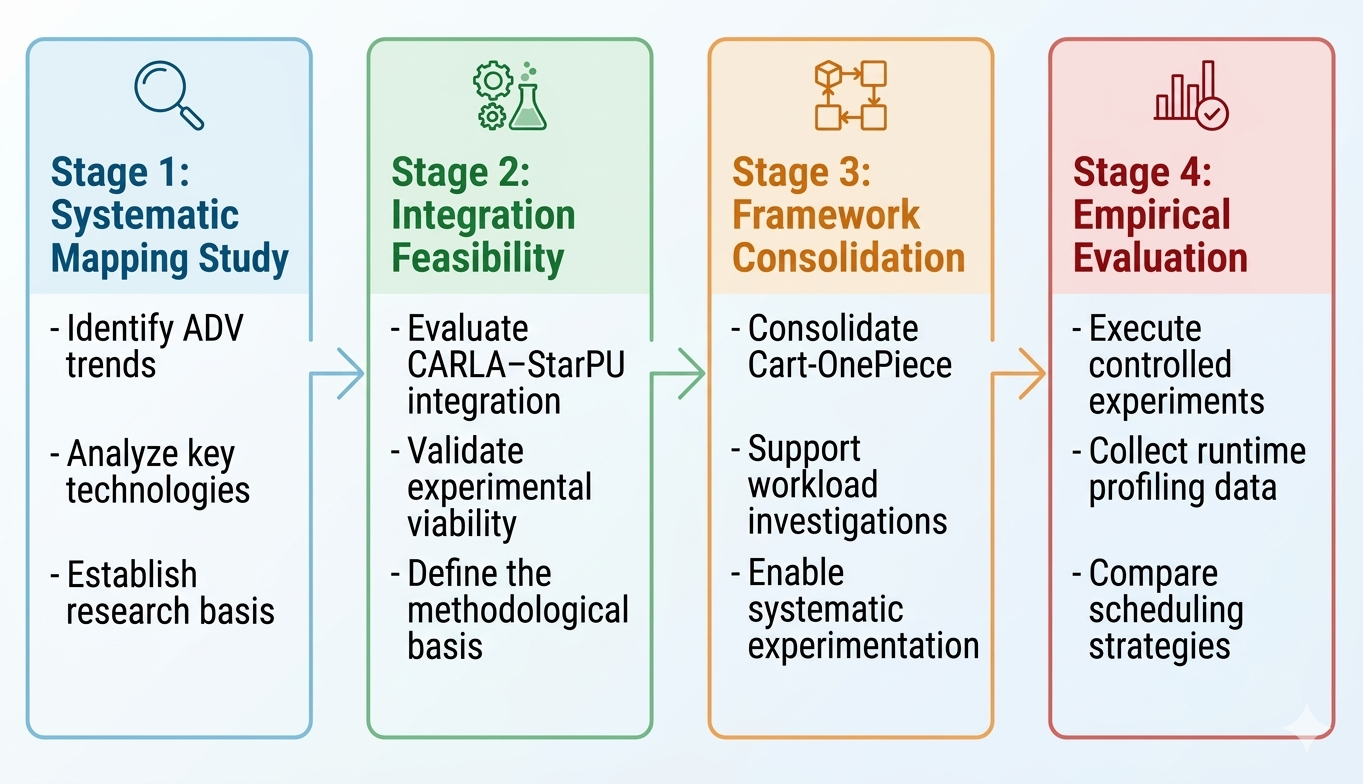
\includegraphics[width=1\textwidth]{imagens/Methodology.png}
  \captionsetup{justification=centering}
  \captionfont{\small{\textbf{\\Source: Elaborated by the author}}}  
  \label{fig:methods}
\end{figure}



The first methodological stage consisted of a systematic mapping study of autonomous vehicles. Rather than serving only as a bibliographic background, this stage provided the analytical foundation for the thesis by identifying technological trends, recurring hardware and software choices, and the sensor configurations most frequently associated with advanced autonomous driving systems. Most of the results found in this step are presented in the background section and also generated a paper published by this theses author. \cite{silva2024}%In methodological terms, this stage was important because it delimited the technological space of interest and provided objective criteria for later decisions regarding which type of computational infrastructure and perception context should be represented in the experimental environment.

The analysis revealed that the heterogeneity of modern processing platforms (coupling CPUs, GPUs, and distinct accelerators) and the need to efficiently process multimodal sensor data impose significant challenges for ADV development. Consequently, it highlighted the need to integrate robust simulation environments with advanced runtime resource managers as a safe and effective path to explore these computational constraints.

The second stage corresponded to the transition from analytical understanding to experimental feasibility. At this point, the research has been moved to evaluate the integration of CARLA and StarPU. The purpose of this stage was not yet to provide a complete benchmarking framework but to verify whether a realistic simulation environment could be combined with a runtime system in a way that enabled the observation of scheduling behavior and workload analyzes. Therefore, this stage functioned as a methodological validation of the core integration on which the later phases of the thesis were built. This step generated a publication that covers the initial attempts of working with the integration focusing on task scheduling analyzes of a simple visual processing of cameras in an ADV. \cite{Silva2025TaskRuntime}

With this feasibility established, the method advanced to a third stage in which the scope of the study was expanded and consolidated in the Cart-OnePiece framework. In this stage, the methodological emphasis shifted from integration alone to the organization of a broader research instrument capable of supporting three complementary activities: the generation of datasets, the characterization of computational workload, and the benchmarking and creation of task scheduling strategies. During this development, a big study of the state of the art of these three main areas explored by CArt-OnePiece was carried out and presented in the state of the art section. This transition is central to the thesis method because it transforms the environment from a proof of concept into a structured platform for systematic empirical investigation. 

Based on this trajectory, the final method adopted in the thesis consists of using the developed infrastructure as an experimental instrument in controlled simulation scenarios. The study is organized so that autonomous driving workloads can be instantiated under repeatable conditions, observed through runtime and profiling data, and compared under different scheduling strategies. In this step, it was found that the tool would also be useful to apply AI algorithms and engines related to ADV to be validated and tested in the CArt-OnePiece application, which was not foreseen in the begging of the development. In this way, the method links the earlier analytical stages of the research to the empirical evaluation stage, allowing the thesis to move from understanding the domain to constructing the investigative environment, and finally to examining how workload behavior and scheduling choices interact in heterogeneous ADV computing systems. 

